% Options for packages loaded elsewhere
\PassOptionsToPackage{unicode}{hyperref}
\PassOptionsToPackage{hyphens}{url}
\PassOptionsToPackage{dvipsnames,svgnames,x11names}{xcolor}
%
\documentclass[
]{report}

\usepackage{amsmath,amssymb}
\usepackage{iftex}
\ifPDFTeX
  \usepackage[T1]{fontenc}
  \usepackage[utf8]{inputenc}
  \usepackage{textcomp} % provide euro and other symbols
\else % if luatex or xetex
  \usepackage{unicode-math}
  \defaultfontfeatures{Scale=MatchLowercase}
  \defaultfontfeatures[\rmfamily]{Ligatures=TeX,Scale=1}
\fi
\usepackage{lmodern}
\ifPDFTeX\else  
    % xetex/luatex font selection
\fi
% Use upquote if available, for straight quotes in verbatim environments
\IfFileExists{upquote.sty}{\usepackage{upquote}}{}
\IfFileExists{microtype.sty}{% use microtype if available
  \usepackage[]{microtype}
  \UseMicrotypeSet[protrusion]{basicmath} % disable protrusion for tt fonts
}{}
\makeatletter
\@ifundefined{KOMAClassName}{% if non-KOMA class
  \IfFileExists{parskip.sty}{%
    \usepackage{parskip}
  }{% else
    \setlength{\parindent}{0pt}
    \setlength{\parskip}{6pt plus 2pt minus 1pt}}
}{% if KOMA class
  \KOMAoptions{parskip=half}}
\makeatother
\usepackage{xcolor}
\setlength{\emergencystretch}{3em} % prevent overfull lines
\setcounter{secnumdepth}{-\maxdimen} % remove section numbering
% Make \paragraph and \subparagraph free-standing
\ifx\paragraph\undefined\else
  \let\oldparagraph\paragraph
  \renewcommand{\paragraph}[1]{\oldparagraph{#1}\mbox{}}
\fi
\ifx\subparagraph\undefined\else
  \let\oldsubparagraph\subparagraph
  \renewcommand{\subparagraph}[1]{\oldsubparagraph{#1}\mbox{}}
\fi


\providecommand{\tightlist}{%
  \setlength{\itemsep}{0pt}\setlength{\parskip}{0pt}}\usepackage{longtable,booktabs,array}
\usepackage{calc} % for calculating minipage widths
% Correct order of tables after \paragraph or \subparagraph
\usepackage{etoolbox}
\makeatletter
\patchcmd\longtable{\par}{\if@noskipsec\mbox{}\fi\par}{}{}
\makeatother
% Allow footnotes in longtable head/foot
\IfFileExists{footnotehyper.sty}{\usepackage{footnotehyper}}{\usepackage{footnote}}
\makesavenoteenv{longtable}
\usepackage{graphicx}
\makeatletter
\def\maxwidth{\ifdim\Gin@nat@width>\linewidth\linewidth\else\Gin@nat@width\fi}
\def\maxheight{\ifdim\Gin@nat@height>\textheight\textheight\else\Gin@nat@height\fi}
\makeatother
% Scale images if necessary, so that they will not overflow the page
% margins by default, and it is still possible to overwrite the defaults
% using explicit options in \includegraphics[width, height, ...]{}
\setkeys{Gin}{width=\maxwidth,height=\maxheight,keepaspectratio}
% Set default figure placement to htbp
\makeatletter
\def\fps@figure{htbp}
\makeatother

\usepackage{booktabs}
\usepackage{amsthm}
\usepackage{placeins}
\makeatletter
\def\thm@space@setup{%
  \thm@preskip=8pt plus 2pt minus 4pt
  \thm@postskip=\thm@preskip
}
\makeatother
\usepackage{adjustbox}
\usepackage{awesomebox}
\usepackage{color}
\usepackage{framed}
\setlength{\fboxsep}{.8em}
\usepackage[most]{tcolorbox}
\usepackage{blindtext}
\usepackage{amsmath}
\usepackage{amssymb}
\usepackage{bm}
\usepackage[finnish]{babel}
\usepackage{graphicx}
\usepackage{placeins}
\usepackage{overpic}
\usepackage{lmodern}
\usepackage{epsfig}
\usepackage{placeins}
\usepackage{xstring}     % Used for \IfEqCase


\definecolor{myboxcolor}{named}{blue} % Default box color

\definecolor{my-purple}{RGB}{204,180,225}
\newtcolorbox{defblock}[1]{%
    breakable,
    enhanced,
    coltext=black,
    colback=my-purple,      % Box color is used here
    colframe=myboxcolor!25!my-purple,     % Box color is used here
    detach title,
    after upper={\par\hfill\tcbtitle}        % Box title is used here 
}

\definecolor{my-orange}{RGB}{255,205,138}
\newtcolorbox{eblock}[1]{%
    breakable,
    enhanced,
    coltext=black,
    colback=my-orange,      % Box color is used here
    colframe=myboxcolor!25!my-orange,     % Box color is used here
    detach title,
    after upper={\par\hfill\tcbtitle}        % Box title is used here 
}


\newcommand{\Rspace}{\mathcal{R}}

\newcommand{\N}{\mathsf{N}}
\newcommand{\Cov}{\mathsf{Cov}}

\newcommand{\Prob}{\mathsf{P}}

\newcommand{\X}{\textbf{X}} 
\newcommand{\Y}{\textbf{Y}} 
\newcommand{\x}{\textbf{x}}                                   
\newcommand{\y}{\textbf{y}}  
\newcommand{\boldc}{\textbf{c}} 
\newcommand{\boldd}{\textbf{d}}  
\newcommand{\bolda}{\textbf{a}}  
\newcommand{\THETA}{\mx{\theta}}
\newcommand{\PHI}{\mx{\phi}}                                   
\newcommand{\VAREPSILON}{\mx{\varepsilon}}                                   
\newcommand{\hatVAREPSILON}{\mx{\hat{\VAREPSILON}}}
\newcommand{\boldP}{\textbf{P}}
\newcommand{\boldM}{\textbf{M}}
\newcommand{\z}{\mx{z}}
\newcommand{\A}{\textbf{A}}
\newcommand{\C}{\textbf{C}}
\newcommand{\hatMU}{\mx{\hat{\mu}}}
\newcommand{\SIGMA}{\mx{\Sigma}}
\newcommand{\ZERO}{\mx{0}}
\newcommand{\ONE}{\mx{1}}
\newcommand{\diag}{\textbf{I}}

\newcommand{\bl}[1]{\textcolor{blue}{#1}}
\newcommand{\rd}[1]{\textcolor{red}{#1}}
\newcommand{\gr}[1]{\textcolor{darkgreenx}{#1}}


%\newcommand\indep{\protect\mathpalette{\protect\independenT}{\perp}}
%\def\independenT#1#2{\mathrel{\rlap{$#1#2$}\mkern2mu{#1#2}}}
\makeatletter
\makeatother
\makeatletter
\makeatother
\makeatletter
\@ifpackageloaded{caption}{}{\usepackage{caption}}
\AtBeginDocument{%
\ifdefined\contentsname
  \renewcommand*\contentsname{Table of contents}
\else
  \newcommand\contentsname{Table of contents}
\fi
\ifdefined\listfigurename
  \renewcommand*\listfigurename{List of Figures}
\else
  \newcommand\listfigurename{List of Figures}
\fi
\ifdefined\listtablename
  \renewcommand*\listtablename{List of Tables}
\else
  \newcommand\listtablename{List of Tables}
\fi
\ifdefined\figurename
  \renewcommand*\figurename{Figure}
\else
  \newcommand\figurename{Figure}
\fi
\ifdefined\tablename
  \renewcommand*\tablename{Table}
\else
  \newcommand\tablename{Table}
\fi
}
\@ifpackageloaded{float}{}{\usepackage{float}}
\floatstyle{ruled}
\@ifundefined{c@chapter}{\newfloat{codelisting}{h}{lop}}{\newfloat{codelisting}{h}{lop}[chapter]}
\floatname{codelisting}{Listing}
\newcommand*\listoflistings{\listof{codelisting}{List of Listings}}
\makeatother
\makeatletter
\@ifpackageloaded{caption}{}{\usepackage{caption}}
\@ifpackageloaded{subcaption}{}{\usepackage{subcaption}}
\makeatother
\makeatletter
\@ifpackageloaded{tcolorbox}{}{\usepackage[skins,breakable]{tcolorbox}}
\makeatother
\makeatletter
\@ifundefined{shadecolor}{\definecolor{shadecolor}{rgb}{.97, .97, .97}}
\makeatother
\makeatletter
\makeatother
\makeatletter
\makeatother
\ifLuaTeX
  \usepackage{selnolig}  % disable illegal ligatures
\fi
\IfFileExists{bookmark.sty}{\usepackage{bookmark}}{\usepackage{hyperref}}
\IfFileExists{xurl.sty}{\usepackage{xurl}}{} % add URL line breaks if available
\urlstyle{same} % disable monospaced font for URLs
\hypersetup{
  pdftitle={Luku 6 - Otokset ja otosjakaumat: tilastollisen päättelyn näkökulma},
  colorlinks=true,
  linkcolor={blue},
  filecolor={Maroon},
  citecolor={Blue},
  urlcolor={Blue},
  pdfcreator={LaTeX via pandoc}}

\title{Luku 6 - Otokset ja otosjakaumat: tilastollisen päättelyn
näkökulma}
\usepackage{etoolbox}
\makeatletter
\providecommand{\subtitle}[1]{% add subtitle to \maketitle
  \apptocmd{\@title}{\par {\large #1 \par}}{}{}
}
\makeatother
\subtitle{Tiivistelmä}
\author{}
\date{}

\begin{document}
\maketitle
\ifdefined\Shaded\renewenvironment{Shaded}{\begin{tcolorbox}[enhanced, frame hidden, breakable, interior hidden, boxrule=0pt, borderline west={3pt}{0pt}{shadecolor}, sharp corners]}{\end{tcolorbox}}\fi

\hypertarget{luvun-ydinviesti}{%
\section{Luvun ydinviesti}\label{luvun-ydinviesti}}

Tässä luvussa tarkastellaan otoksia ja otosjakaumia ``tilastollisemmin''
mitä edellisten erityisesti otantaa koskevan johdannan yhteydessä,
toisin sanoen nyt tutustumme kevyesti tilastolliseen päättelyyn!

Tämä luku on kurssin materiaalista matemaattisin, mutta siitä ei tule
huolestua. Tavoite on yhdistää aiemmin opittuja konsepteja
matemaattiseen merkintätapaan.

Tilastolliseen päättelyyn perehdytään tarkemmin tilastollisen päättelyn
peruskurssilla
(\href{https://opas.peppi.utu.fi/fi/opintojakso/TILM3555/1731}{TILM3555})

Ydinviestinä olkoon siis matemaattisen formaalin esitystavan
yhdistäminen aiemmin opittuihin konsepteihin! Uutena asiana puhutaan
hieman aineistosta laskettaviin tunnuslukuihin ja estimaattoreihin.

\hypertarget{satunnaisotos-yhteisjakauma-ja-tilastollinen-malli}{%
\section{Satunnaisotos, yhteisjakauma ja tilastollinen
malli}\label{satunnaisotos-yhteisjakauma-ja-tilastollinen-malli}}

Satunnaismuuttujilla on todennäköisyysjakaumat, joita tilastotieteessä
kuvataan todennäköisyys- eli tiheysfunktion (tai
pistetodennäköisyysfunktion) avulla.

\begin{defblock}{}
\textbf{Satunnaisotos}

Olkoot \(Y_1, \dots, Y_n\) riippumattomia ja samoinjakautuneita
satunnaismuuttujia, joiden tiheysfunktiota (tf., tai
pistetodennäköisyysfunktiota (ptnf)) merkitään \(f(y,\theta)\):llä,
jossa \(y\) on yksittäisen sm:jan \(Y\):n realisaatio ja \(\theta\) on
jokin jakauman muodon määräävä parametri (tai parametrit).

Parametrin \(\theta\) arvoa ei yleensä tunneta ja tavoitteena onkin
päätellä, \textbf{estimoida}, sen arvo lopulta käytettävissä olevasta
aineistosta.

\end{defblock}

\hypertarget{satunnaisotoksen-tilastollinen-malli}{%
\section{Satunnaisotoksen tilastollinen
malli}\label{satunnaisotoksen-tilastollinen-malli}}

Satunnaismuuttujien havaitut arvot muodostavat siis satunnaisotoksen. Ne
ovat kiinteitä lukuja, mutta vaihtelevat satunnaisesti otoksesta
toiseen.

Täten satunnaisotannassa \textbf{satunnaisuus liittyy siis
havaintoarvojen vaihteluun satunnaisesti otoksesta toiseen.
Tilastollinen malli} on näiden havaintoarvojen otosten välistä vaihtelua
kuvaava \textbf{yhteisjakauma}.

Edellä oletettiin että satunnaismuuttujat ovat keskenään riippumattomia,
jolloin tämä yhteisjakauma on seuraavaa tulomuotoa
\(f(y_1,\dots,y_n;\theta) = f(y_1;\theta) \times \cdots \times f(y_n;\theta)\)

Tilastollinen mallin muoto riippuu tutkijan tekemästä
jakaumaoletuksesta, jonka monimutkaisuus ilmenee sen parametrien
määrästä. Niin sanotun \textbf{parsimoonisuus-} eli
\textbf{vähäparametrisuusperiatteen} mukaan tilastollisen mallin tulisi
olla niin yksinkertainen, eli vähäparametrinen, kuin mahdollista
satunnaisotoksen riittävään kuvaamiseen.

\hypertarget{otosjakauma-klassisen-tilastotieteen-nuxe4kuxf6kulma}{%
\section{Otosjakauma: klassisen tilastotieteen
näkökulma}\label{otosjakauma-klassisen-tilastotieteen-nuxe4kuxf6kulma}}

Ajatus aineiston keruun toistamisesta ilmentää klassisen
(frekventistisen) tilastotieteen käsitystä tilastollisesta
stabiliteetista, jolle tilastollinen päättely perustuu.

Keskeistä tälle on tilastolliseen malliin \(f(y_1,\dots,y_n;\theta)\)
liitetty jakaumaoletus. Mikäli kerättäisiin uusi satunnaisotos, eli
toistettaisiin aineiston keruu, niin satunnaismuuttujien havaitut arvot,
havaintoarvot, vaihtelisivat tilastollisen mallin jakauman kuvaamalla
tavalla!

\hypertarget{otosjakauma-estimaattori-ja-estimaatti}{%
\section{Otosjakauma: Estimaattori ja
estimaatti}\label{otosjakauma-estimaattori-ja-estimaatti}}

Satunnaisotoksesta voidaan laskea erilaisia
\textbf{tunnuslukuja/otossuureita,} joita merkitään
\(T = g(Y_1,\dots,Y_n)\), ts. ne ovat aineiston funktioita. Tunnusluvut
ovat \textbf{satunnaismuuttujien funktioina myös satunnaismuuttujia.}

Tunnusluvuilla on täten myös havaittu arvo satunnaisotoksen määräämässä
pisteessä, merkitään \(t=g(y_1,\dots,y_n)\). Tilastollisen tutkimuksen
tavoite on pyrkiä aineiston avulla arvioimaan, estimoimaan, tunnusluvun
nk. \textbf{todellinen arvo}, \(g(\theta)\).

Koska tunnusluku/estimaattori \(T\) on satunnaismuuttuja, sillä on
todennäköisyysjakauma, jota kutsutaan tunnusluvun \(T\) otosjakaumaksi
ja joka myös riippuu tuntemattomista parametreista.

\hypertarget{keskeiset-termit-harhattomuus}{%
\section{Keskeiset termit:
harhattomuus}\label{keskeiset-termit-harhattomuus}}

\begin{defblock}{}

\textbf{Harhattomuus}

Estimaattorin odotettavissa oleva arvo yhtyy tuntemattoman parametrin
todelliseen arvoon eli \(E(\widehat{\theta}) = \theta\).

\begin{itemize}
\item
  Harhaton estimaattori tuottaa keskimäärin oikean kokoisia arvoja
  (estimaatteja) estimoitavalle parametrille.
\item
  Estimaattorin tuottama arvo, estimaatti, parametrille saattaa
  vaihdella otoksesta toiseen paljonkin, mutta odotusarvon
  frekvenssitulkinnan mukaan otoskohtaiset estimaatit jakautuvat otantaa
  toistettaessa (symmetrisesti) parametrin todellisen arvon ympärille.
\end{itemize}

\end{defblock}

\hypertarget{keskeiset-termit-tyhjentuxe4vyys-tehokkuus-ja-tarkentuvuus}{%
\section{Keskeiset termit: tyhjentävyys, tehokkuus ja
tarkentuvuus}\label{keskeiset-termit-tyhjentuxe4vyys-tehokkuus-ja-tarkentuvuus}}

\begin{defblock}{}
\textbf{Tyhjentävyys}

Tyhjentävä estimaattori käyttää kaiken otokseen sisältyvän parametria
\(\theta\) koskevan informaation.

\end{defblock}

\begin{defblock}{}
\textbf{Tehokkuus}

Kahdesta saman parametrin \(\theta\) estimaattorista tehokkaampi on se,
jonka varianssi on pienempi.

\end{defblock}

\begin{defblock}{}
\textbf{Tarkentuvuus}

Tarkentuvan estimaattorin \(\widehat{\theta}\) arvot lähestyvät
parametrin \(\theta\) oikeaa arvoa otoskoon kasvaessa.

\end{defblock}

\hypertarget{otoskeskiarvo-estimaattorina}{%
\section{Otoskeskiarvo
estimaattorina}\label{otoskeskiarvo-estimaattorina}}

Olkoon \(Y_1,\dots,Y_n\) riippumattomia ja samoinjakautuneita sm:jia, ja
että kyseisen jakauman odotusarvo on \(E(Y_i) = \mu\) ja varianssi
\(\text{Var}(Y_i) = \sigma^2\).

\begin{itemize}
\item
  Satunnaismuuttujien (aritmeettinen) keskiarvo on
  \(\bar{Y} = \frac{1}{n}(Y_1 + \cdots + Y_n) = \frac{1}{n} \sum_{i=1}^n Y_i\)
  ja sitä vastaa otoskeskiarvo
  \(\bar{y} = \frac{1}{n}\sum_{i=1}^n y_i\).
\item
  Kun satunnaismuuttujat ovat samoin jakautuneet odotusarvonaan \(\mu\),
  on otoskeskiarvo jakauman odotusarvon harhaton estimaattori, ts.
  \(E(\bar{Y}) = \mu\) .
\end{itemize}

Tällöin keskiarvo \(\bar{Y}\) on tunnusluku, jota käytetään odotusarvon
estimoimiseen, eli se on estimaattori ja täten sillä on myös jakauma,
jota kuvaa odotusarvo \(E(\bar{Y}) = \mu\) ja varianssi
\(\text{Var}(\bar{Y}) = \frac{\sigma^2}{n}\). Huomataan, että otoskoon
kasvaessa keskiarvon otosjakauma keskittyy yhä voimakkaammin odotusarvon
ympärille.

\hypertarget{otosvarianssi-estimaattorina}{%
\section{Otosvarianssi
estimaattorina}\label{otosvarianssi-estimaattorina}}

Perusjoukon tasolla sm:jien vaihtelua kuvataan
\textbf{populaatiovarianssilla}
\(\sigma^2 = \frac{1}{N}\sum_{j=1}^N(Y_j - \mu)^2\) ja sen aineistosta
laskettava vastine on \textbf{otosvarianssilla}
\(S^2 = \frac{1}{n-1}\sum_{i=1}^n(y_i - \bar{y})^2\).

Huomaa että \textbf{otosvarianssi} on eri asia kuin
\textbf{otoskeskiarvon varianssi.}

Otoskeskiarvo ja otosvarianssi ovat siis satunnaismuuttujia, joiden
saamat arvot vaihtelevat satunnaisesti otoksesta toiseen. Näitä
tunnuslukuja käytetään arvioimaan perusjoukon, eli populaation,
odotusarvoa ja varianssia, joten ne ovat myös estimaattoreita.

\hypertarget{normaalijakautunut-otos}{%
\section{Normaalijakautunut otos}\label{normaalijakautunut-otos}}

Jos satunnaisotoksen muodostavat havainnot \(Y_1,\dots,Y_n\) ovat
peräisin normaalijakaumasta, niin voidaan osoittaa että havaintojen
keskiarvo on myös normaalisti jakautunut, merkitään
\(\bar{Y} \sim \text{N}(\mu, \frac{\sigma^2}{n})\).

Ns. \textbf{asymptoottiseen teoriaan} vedoten voidaan osoittaa että tämä
pätee myös ilman normaalisuusoletusta kun otoskoko on suuri.

\href{https://onlinestatbook.com/stat_sim/sampling_dist/}{Esimerkki}

Standardoitu keskiarvo saadaan vähentämällä keskiarvosta odotusarvo ja
jakamalla se keskipoikkeamalla, merkitään
\(Z = \frac{\bar{Y} - E(\bar{Y})}{D(\bar{Y}} = \frac{\bar{Y} - \mu}{\sigma/\sqrt{n}} = \sqrt{n} \Big( \frac{\bar{Y} - \mu}{\sigma} \Big)\).
Tällöin \(Z\):n odotusarvo \(E(Z)=0\) ja varianssi \(\text{Var}(Z)=1\).
Lisäksi, jos \(Y_i \sim N(\mu,\sigma^2), i=1,\dots,n\), niin \(Z\)
noudattaa standardoitua normaalijakauma \(Z \sim N(0,1)\).

\hypertarget{suhteellisen-frekvenssin-otosjakauma}{%
\section{Suhteellisen frekvenssin
otosjakauma}\label{suhteellisen-frekvenssin-otosjakauma}}

Ohitetaan tiivistelmässä.

\hypertarget{muita-tunnuslukuja}{%
\section{Muita tunnuslukuja}\label{muita-tunnuslukuja}}

Tilastollisessa tutkimuksessa hyödynnetään myös paljon muita otoksesta
laskettavia tunnuslukuja. Erilaiset tunnusluvut kertovat muuttujan
jakaumasta erilaisia asioita, joiden avulla taustalla olevan
satunnaisilmiön luonnetta on helpompi hahmottaa.

\begin{itemize}
\item
  \textbf{Moodi} eli tyyppiarvo on havaintoaineiston yleisin muuttujan
  arvo tai se luokka, jolla on suurin frekvenssi.
\item
  \textbf{Mediaani} on järjestetyn havaintoaineiston keskimmäinen arvo.
  Puolet arvoista on mediaania pienempiä ja puolet suurempia.
\item
  \textbf{Fraktiili} on vastaavasti jotain prosenttiosuutta vastaava
  arvo, joka jakaa aineiston kahteen osaan siten että kyseistä
  fraktiilia vastaavaa havaintoarvoa pienempiä arvoja on kyseinen
  prosenttiosuus.

  \begin{itemize}
  \tightlist
  \item
    Esimerkkeinä \textbf{kvartiilit,} jotka jakavat aineiston 25\%
    välein, ts. \(Q_1\) on ns. alakvartiili, joka vastaa 25\% fraktiilia
    ja yläkvartiili \(Q_3\) on 75\% fraktiili. Näiden erotusta kutsutaan
    \textbf{kvartiiliväliksi} \(=(Q_1,Q_3)\).
  \end{itemize}
\item
  \textbf{Vinous} ja \textbf{huipukkuus} kuvaavat jakauman muotoa,
  erityisesti sen poikkeamaa normaalijakaumasta.
\end{itemize}

\hypertarget{luottamusvuxe4lit}{%
\section{Luottamusvälit}\label{luottamusvuxe4lit}}

Satunnaisotoksesta laskettujen tunnuslukujen luotettavuus on
tilastollisen mallin parametrien estimoinnissa keskeinen kysymys.

\begin{itemize}
\item
  Otantaan liittyvän satunnaisvaihtelun vuoksi emme voi varmuudella
  tietää onko otoksesta laskettu parametriestimaatti ``lähellä'' vai
  ``kaukana'' sen todelisesta arvosta.
\item
  Tätä luotettavuutta voidaan arvioida \textbf{luottamusvälin} avulla.
\end{itemize}

\begin{defblock}{}
\textbf{Luottamusväli}

Luottamusväli on otoksen perusteella määrätty väli, joka tutkijan
valitsemalla todennäköisyydellä (luottamustasolla) peittää
tarkasteltavan tilastollisen mallin \(f(y;\theta)\) parametrin
\(\theta\) tuntemattoman todellisen arvon. Se perustetaan
otostunnusluvun, estimaattorin, otosjakaumaan.

\end{defblock}

\hypertarget{luottamusvuxe4li}{%
\section{Luottamusväli}\label{luottamusvuxe4li}}

\textbf{Luottamustasoa} merkitään usein \(1-\alpha\):lla, jossa
\(\alpha\) on \textbf{merkitsevyystaso} (\textbf{riskitaso}), usein
esimerkiksi \(\alpha = 0.05\). Luottamustaso tulkitaan niin, että jos
\textbf{otantaa} jakaumasta \(f(y;\theta)\) toistetaan, niin keskimäärin
\(100 \times (1-\alpha)\%\) otoksista muodostetuista (konstruloiduista)
luottamusväleistä peittää parametrin \(\theta\) todellisen arvon.

Luottamusväli on tunnetumpi kansankieliseltä nimitykseltään
\textbf{virhemarginaali,} joka on itse asiassa luottamusvälin puolikas.
Todellinen parametriarvo kuuluu saadun estimaatin ja virhemarginaalien
sisään jäävälle osuudelle.

\begin{itemize}
\tightlist
\item
  Virhemarginaalin suuruuteen vaikuttavat otosasetelma, otoskoko,
  luottamustaso ja tutkittavan tilastollisen tunnusluvun jakauma.
\end{itemize}

\hypertarget{normaalijakauman-odotusarvon-luottamusvuxe4li}{%
\section{Normaalijakauman odotusarvon
luottamusväli}\label{normaalijakauman-odotusarvon-luottamusvuxe4li}}

Tarkastellaan seuraavaksi lyhyesti normaalijakauman odotusarvon
luottamusvälejä silloin kun taustalla oleva populaatio on ``iso''
(ääretön).

Tarkastellaan satunnaisotosta normaalijakaumasta \(Y_1,\dots,Y_n\),
missä satunnaismuuttujat ovat riippumattomia ja niille pätee
\(Y_i \sim N(\mu,\sigma^2)\).

Muistetaan että keskiarvo on normaalijakauman odotusarvoparametrin
\textbf{harhaton estimaattori}
\(\bar{Y} = \frac{1}{n}\sum_{i=1}^n Y_i\).

Valitaan \textbf{luottamustasoksi} \(1-\alpha\), eli \(\alpha\) määrää
todennäköisyyden, jolla luottamusväli peittää odotusarvon \(\mu\)
todellisen arvon. Yleinen valinta ihmistieteissä on \(\alpha = 0.05\)
tai \(\alpha = 0.1\) vastaten 95\% ja 90\% luottamustasoa.
Luonnotieteissä \(\alpha\) on usein paljon pienempi.

\hypertarget{normaalijakauman-odotusarvon-luottamusvuxe4li-1}{%
\section{Normaalijakauman odotusarvon
luottamusväli}\label{normaalijakauman-odotusarvon-luottamusvuxe4li-1}}

Seuraavaksi määrätään \textbf{luottamuskertoimet} \(-z_{\alpha/2}\) ja
\(z_{\alpha/2}\), joille pätee
\(P(-z_{\alpha/2} \leq Z \leq z_{\alpha/2}) = 1 - \alpha\), jossa \(Z\)
on standardoitu satunnaismuuttuja ja noudattaa \(N(0,1)\) jakaumaa
(standardinormaalijakaumaa).

Sijoitetaan standardoidun satunnaismuuttujan määritelmä yo.
epäyhtälöketjuun ja saadaan

\(-z_{\alpha/2} \le \frac{\bar{Y} - \mu}{\sigma / \sqrt{n}} \le z_{\alpha/2}\),

joka voidaan kirjoittaa uudelleen muodossa

\(\bar{Y} - z_{\alpha/2} \frac{\sigma}{\sqrt{n}} \le \mu \le \bar{Y} + z_{\alpha/2} \frac{\sigma}{\sqrt{n}}\)

Normaalijakauman odotusarvon \((1-\alpha)\times 100\%\) luottamusväli on
siis

\(\Big(\bar{Y} - z_{\alpha/2} \frac{\sigma}{\sqrt{n}}, \bar{Y} + z_{\alpha/2} \frac{\sigma}{\sqrt{n}} \Big).\)

\hypertarget{luottamustason-tulkinta}{%
\section{Luottamustason tulkinta}\label{luottamustason-tulkinta}}

Miten luottamustasoa \((1-\alpha)\) tulisi tulkita? Olisi toivottavaa,
että estimoidulle parametrille pystyttäisiin konstruoida mahdollisimman
lyhyt luottamusväli, sillä tämä tarkoittaisi että saatu estimaatti olisi
luotettavampi!

Samanaikaisesti olisi toivottavaa, että luottamustaso olisi
mahdollisimman korkea, sillä tämä tarkoittaa nimensä mukaisesti saatu
estimaatti olisi luotettavampi!

Molempien vaatimusten samanaikainen täyttäminen ei ole kuitenkaan
mahdollista, jos otoskoko \(n\) pidetään kiinteänä:

\begin{itemize}
\item
  Luottamustason kasvattaminen pidentää luottamusväliä, jolloin tieto
  parametrin \(\mu\) todellisesta arvosta tulee epätarkemmaksi.
\item
  Luottamusvälin lyhentäminen pienentää luottamustasoa, jolloin tieto
  parametrin \(\mu\) todellisesta arvosta tulee epävarmemmaksi.
\end{itemize}

\hypertarget{luottamustason-tulkinta-graafisesti}{%
\section{Luottamustason tulkinta
graafisesti}\label{luottamustason-tulkinta-graafisesti}}

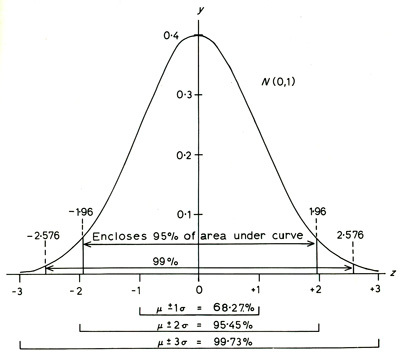
\includegraphics[width=3.6875in,height=\textheight]{gaussian-distribution.jpg}

\hypertarget{otoskoko}{%
\section{Otoskoko}\label{otoskoko}}

Kuten jo tiedetään, yksi tilastollisen tutkimuksen (päättelyn) keskeisiä
tavoitteita on yleistää otoksen pohjalta tehty päättely koskemaan koko
perusjoukkoa.

\begin{itemize}
\item
  Kun otoskoko on liian pieni, voi otos \textbf{sattumalta} poiketa
  paljonkin perusjoukosta.
\item
  Todella suuren otoksen kerääminen/koostaminen voi olla
  \textbf{työlästä, kallista} tai joskus jopa \textbf{täysin
  mahdotonta!}
\end{itemize}

Toisaalta otoskoon kasvaessa perusjoukon systemaattiset piirteet tulevat
paremmin esille, eli se vaikuttaa keskeisesti siihen miten hyvin
otoksesta tehdyt johtopäätökset voidaan yleistää perusjoukolle.

Onneksi on usein mahdollista määrätä etukäteen otoskoko, jolla
tutkimusongelmaan voidaan vastata riittävällä tarkkuudella!

\hypertarget{mitkuxe4-asiat-vaikuttavat-otoskoon-muxe4uxe4rittuxe4miseen}{%
\section{Mitkä asiat vaikuttavat otoskoon
määrittämiseen?}\label{mitkuxe4-asiat-vaikuttavat-otoskoon-muxe4uxe4rittuxe4miseen}}

Käydään seuraavaksi lyhyesti läpi mitkä asiat vaikuttavat otoskoon
määrittämiseen, mutta ohitetaan sen tarkempi käsittely tässä
tiivistelmässä.

\begin{enumerate}
\def\labelenumi{\arabic{enumi}.}
\tightlist
\item
  \textbf{Perusjoukko}. Tutkimusmuuttujien vaihtelu perusjoukossa
  vaikuttaa keskeisesti tarvittavaan otoskokoon. Samoin esimerkiksi
  perusjoukon mahdollinen ryhmärakenne!
\item
  \textbf{Tulosten vaadittu tarkkuus}.

  \begin{enumerate}
  \def\labelenumii{\arabic{enumii}.}
  \tightlist
  \item
    Kuinka varma halutaan olla, että saadut tulokset yleistyvät
    perusjoukkoon? Tämä määrittää virhemarginaalin! Suurempi sallittu
    virhemarginaali tarkoittaa pienempää otoskokoa ja päinvastoin.
  \item
    Kuinka varma haluat olla, että otos edustaa joukkoa oikein? Tämä
    määrittää luottamustason! Suurempi haluttu luottamustaso tarkoittaa
    suurempaa otoskokoa ja päinvastoin.
  \end{enumerate}
\item
  \textbf{Odotetun} \textbf{vastauskadon vaikutus.} Koskee
  kyselytutkimuksia, joissa usein käy niin että osa kyselytutkimukseen
  valituista jättää vastaamatta.
\end{enumerate}



\end{document}
